\NeedsTeXFormat{LaTeX2e}
%-----------------------------------------------------------
\documentclass[a4paper,12pt]{monografia}
\usepackage[brazil]{babel}
\usepackage[utf8]{inputenc}
\usepackage[T1]{fontenc}
\usepackage{indentfirst}
\usepackage{hyphenat}
\usepackage{csquotes}
\usepackage{courier}
\usepackage{graphicx}
\usepackage{listings}
\usepackage{color}
\usepackage[toc,acronym]{glossaries}
\usepackage[backend=biber, style=abnt]{biblatex} 

% !!! SHARELATEX Workaround para referências ABNT (Deve-se colocar os sobrenomes em maiúscula no .bib)
%\usepackage[backend=biber, style=authortitle]{biblatex} % Descomente se estiver usando Sharelatex
\usepackage[hidelinks]{hyperref} % Torna os links da referência clicáveis
\setlength{\bibhang}{0pt}

% === Adição do arquivo de bibliografia
\addbibresource{biblio.bib}
%\renewcommand*{\nameyeardelim}{\addcomma\space} % estilização para citações autor/ano

% === Estilo para trechos de códigos
\definecolor{codebg}{RGB}{240,240,240}
\lstdefinestyle{codigo}{
    backgroundcolor=\color{codebg},
    keywordstyle=\color{blue},
    basicstyle=\footnotesize,
    breakatwhitespace=false,         
    breaklines=true,                 
    captionpos=b,                    
    keepspaces=true,                 
    numbers=left,                    
    numbersep=5pt,                  
    showspaces=false,                
    showstringspaces=false,
    showtabs=false,                  
    tabsize=2
}
 
\lstset{style=codigo}

% === Gerar o glossário e lista de abreviaturas (Opcional)
\makeglossaries
\newacronym{gcd}{GCD}{Greatest Common Divisor}

\newglossaryentry{angelsperarea}{
  name = $a$ ,
  description = The number of angels per unit area,
}


% === Comando para imagens onde se deve destacar a fonte
\newcommand*{\captionsource}[2]{%
  \caption[{#1}]{%
    #1%
    \\\hspace{\linewidth}%
    \textbf{Fonte:} #2%
  }%
}

\begin{document}

% === Título e Dados do Autor 
\titulo{COLOQUE SEU TÍTULO AQUI}
%\subtitulo{Subtítulo} % opcional
\autor{Daniel Barlavento Gomes} \nome{Daniel} \ultimonome{Barlavento Gomes}

% === Curso e Grau
\bacharelado \curso{Tecnologia em Análise e Desenvolvimento de Sistemas} \ano{\textbf{2017}}
\data{04/12/2017} % data da aprovação
\cidade{Recife}
\estado{Pernambuco}

% === Informações sobre a Instituição
\instituicao{INSTITUTO FEDERAL DE EDUCAÇÃO, CIÊNCIA E TECNOLOGIA DE PERNAMBUCO} \sigla{IFPE}
\unidadeacademica{DEPARTAMENTO ACADÊMICO DE SISTEMA, PROCESSOS E CONTROLES ELETRO-ELETRÔNICO}

% === Informações obtidas na Biblioteca
%\CDU{XXX.XX} \areas{1.???  2.???}
%\npaginas{xx}  % total de páginas do trabalho

% === Nomes do Orientador, 1o. Examinador Interno e 2o. Examinador Externo
\orientador{Paulo Abadie Guedes}
%\coorientador{Nome do Co-orientador} % opcional

\examinadorum{Examinador Interno 1}
\examinadordois{Examinador Externo 2}
%\examinadortres{Nome do Examinador 3}
%\examinadorquatro{Nome do Examinador 4}

% === Títulos do Orientador, 1o. e 2o. Examinadores
\ttorientador{Mestre}
%\ttcoorientador{Título do Co-orientador} % se digitado \coorientador

\ttexaminadorum{Doutor}
\ttexaminadordois{Doutor}
%\ttexaminadortres{Título do Examinador 3}
%\ttexaminadorquatro{Título do Examinador 4}

% === Funções do 1o. e 2o. Examinadores
\funcaoexaminadorum{Professor do Instituto Federal de Pernambuco}
\funcaoexaminadordois{Professor do Curso de Sistemas de Informações da Universidade}

\maketitle

% === Dedicatória (Opcional)
\begin{dedicatoria}
Dedico a  minha família, por todo o apoio e confiança.
\end{dedicatoria}
\maketitle

% === Agradecimentos (Opcional)
%\agradecimento{AGRADECIMENTOS}
% Digite seu texto de agradecimento aqui
%\newpage
% ou inclua um arquivo .tex como mostrado abaixo
\agradecimento{AGRADECIMENTOS}%
\newpage

% === Epígrafe (Opcional)
\begin{epigrafe}
``Prefiro não fazer''.\\
\hfill Herman Melville (Bartleby, o escriturário)
\end{epigrafe}

% === Inclua seu resumo em Português
%\resumo{Resumo}
% Digite seu resumo aqui
%\noindent Palavras-chave:
% ou inclua um arquivo .tex como mostrado abaixo
\resumo{RESUMO}
A crescente complexidade dos sistemas de tempo real torna necessária a utilização de técnicas e ferramentas que possibilitem aos projetistas um maior controle das aplicações desenvolvidas, tornem o desenvolvimento estruturado, possibilitem a reutilização de código e proporcionem meios para a manutenção das aplicações. Os sistemas operacionais de tempo real existem para suprir estas necessidades, a maior parte desses sistemas são proprietários e possuem um custo de licenciamento alto. Devido a necessidade de desenvolver um sistema operacional de tempo real de baixo custo diversos projetistas criaram soluções que dessem ao Linux suporte para executar aplicações de tempo real. O \textit{patch} Preempt\_RT, suportado oficialmente pelos desenvolvedores do \textit{kernel} Linux, e o RTAI, uma solução que utiliza uma arquitetura com dois \textit{kernels}, são duas soluções capazes de transformar o Linux em um sistema operacional de tempo real. Neste trabalho as duas soluções foram aplicadas a um sistema Linux que teve seu desempenho medido por meio de um conjunto de testes e os resultados avaliados, afim de verificar a real capacidade do sistema em atender os requisitos de uma aplicação de tempo real.   

\noindent Palavras-chave: Linux de Tempo Real, Sistemas de Tempo Real, Sistemas Operacionais de Tempo Real, Análise de Desempenho, Preempt\_RT, RTAI


% === Digite aqui o seu resumo em Inglês
%\resumo{Abstract}
% Digite seu resumo aqui
%\noindent Keywords:
% ou inclua um arquivo .tex como mostrado abaixo
\resumo{ABSTRACT}
Curabitur malesuada ante lorem, a auctor urna euismod et. Nam viverra, dolor eu feugiat euismod, justo velit tincidunt purus, faucibus interdum mauris metus in turpis. Maecenas hendrerit, felis quis condimentum convallis, metus turpis porttitor ex, non iaculis nisi ex id ligula. Vivamus sed consectetur felis. Maecenas non ligula eu nulla iaculis dictum. Phasellus accumsan tempus purus et consectetur. Praesent dapibus, arcu ut porta dictum, velit lacus ultricies nisl, vitae congue purus mi id ipsum. Pellentesque ac tempus enim, at egestas nulla. Quisque vitae ultrices odio. Lorem ipsum dolor sit amet, consectetur adipiscing elit. Sed vitae purus ultricies, maximus magna a, aliquet mauris. Aliquam ornare odio sit amet urna placerat vestibulum. Aenean a cursus mauris, quis vulputate erat. Nullam convallis scelerisque ligula, at finibus lectus laoreet at. 

\noindent Keywords:

% === Ou digite aqui o seu resumo em Francês
%\resumo{Résumé}
% Digite seu resumo aqui
%\noindent Mots-clés: 
% ou inclua um arquivo .tex como mostrado abaixo
%\input{resume}

% === Lista de figuras(Opcional), lista de tabelas(Opcional), lista de abreviações(Opcional) e sumário
%\listoffigures \thispagestyle{empty}
%\listoftables \thispagestyle{empty}
\printglossary[type=\acronymtype]
\tableofcontents

% !!! Início do Conteúdo
\pagestyle{ruledheader}

% === Hifenização
% Colocar lista de palavras que não devem ser separadas ou que não estão no dicionario português.
\hyphenation{ Hardware Software }

% === Capítulos
% A partir daqui coloque seus capítulos. Sugere-se que eles sejam inseridos com o comando \input
% Da seguinte maneira: (Devem estar na mesma pasta deste arquivo)

\chapter{INTRODUÇÃO}
\label{cap:introducao}
Sistemas de tempo real se tornaram elemento constante na vida das pessoas e estão presentes em locais que vão de aparelhos condicionadores de ar a grandes usinas geradores de energia.

Devido ao aumento da complexidade dos sistemas de tempo real os desenvolvedores veem procurando soluções que permitam a construção destes sistemas de forma rápida, estruturada e que possível de ser mantida a longo prazo, o que sempre foi uma grande dificuldade nos sistemas desenvolvidos  em \textit{assembly}. Devido ao aumento da capacidade de processamento dos processadores atuais, como parte da solução, sistemas operacionais de tempo real vem sendo cada vez mais utilizados no desenvolvimento de novos projetos, pois proporcionam uma grande variedade de funcionalidades previamente implementadas e gerenciam praticamente todo o hardware. 

Grande parte dos sistemas operacionais de tempo real disponíveis no mercado são proprietários, com um alto custo de licenciamento, ou não possuem suporte a recursos mais avançados exigidos por algumas aplicações. Devido a este problema vários projetos foram desenvolvidos com a finalidade de transforma o Linux em um verdadeiro sistema operacional de tempo real. Dentre as soluções criadas podemos destacar o \textit{patch} Preempt\_RT, suportado oficialmente pelos desenvolvedores do \textit{kernel} Linux, e o RTAI uma solução baseada em \textit{microkernel}.

A validação por meio da execução de \textit{benchmarks} da transformação do Linux em um sistema de tempo real utilizando Preempt\_RT e RTAI, fornece uma base sólida de dados que permitem a um projetista de sistemas de tempo real comparar as soluções baseadas em Linux com outros sistemas e verificar se as restrições temporais de seus projetos podem ser atendidas.

A definição, implementação, aplicação de testes a sistemas Linux modificados para suportar aplicações de tempo real e a avaliação, dentre outras características, do desempenho das duas soluções utilizadas, Preempt\_RT e RTAI, a fim de fornecer um conjunto de dados que possam ser úteis, não só na seleção entre sistemas operacionais de tempo real mas uma base sobre a qual avaliações mais aprofundadas possam ser construídas. 


\section{Objetivos}
Este trabalho tem como objetivos gerais e específicos:
\subsection{Gerais}
Este trabalho tem como objetivo avaliar a capacidade do \textit{patch} Preempt\_RT, oficialmente
suportado pelos desenvolvedores do \textit{kernel}, de transformar um PC com um único processador em um
computador capaz atender aos requisitos de uma aplicação de tempo real rígida e comparar os
resultados com o RTAI, um sistema maduro, testado e consolidado.

Para esta avaliação foram escritas duas aplicações, baseadas nos testes realizados por
Anderson(2007) e no \textit{benchmark} Cyclictest, e portadas para o RTAI para que fosse possível realizar a
comparação. Nesse processo também foi observada a facilidade de instalação dos respectivos patch e
desenvolvimento de aplicações para ambas as soluções.
\subsection{Específicos}
\begin{itemize}
    \item Verificar a viabilidade de uso do \textit{patch} Preempt\_RT e do RTAI na máquina de testes e distribuição escolhida
    \item Criação de \textit{kernels} de tempo real baseados nas duas soluções estudadas
    \item Escrita dos testes
    \item Aplicação dos testes
    \item Avaliação dos resultados obtidos
\end{itemize}

\section{Trabalhos relacionados}
Durante a pesquisa bibliográfica foram identificados alguns trabalhos semelhantes e que nos proveram diversos recursos para a elaboração deste trabalho, dentre eles se destacam \cite{Anderson2007}, que nos forneceu o modelo de teste utilizado neste trabalho, assim como medições de performance do RTAI que foram utilizados como valores de referência para verificação dos testes desenvolvidos.

Também podem ser destacados os trabalhos de \cite{Litayem2011} e \cite{Hallberg2017} que forneceram valores de referência e demonstram a real qualidade dos resultados oferecidos pelo \textit{benchmark} Cyclictest na avaliação e comparação de sistemas de tempo real baseados em Linux, embora não deixem muito claro em que circunstâncias os testes forma executados.


\chapter{ESTADO DA ARTE}
\label{cap:estadoarte}

\section{Sistemas de Tempo Real}
\subsection{Conceitos}
\subsection{Classificação}
\subsection{Algoritmos de Escalonamento}

\section{Sistemas Operacionais de Tempo Real}
\subsection{GNU-LINUX}
\subsection{Implementações}

\section{O Projeto PREMPT\_RT}

\section{RTAI}
\chapter{MATERIAIS E MÉTODOS}
\label{cap:projeto}

\section{Avaliação de Sistemas Tempo Real}
A avaliação de um SOTR é definida principalmente pela capacidade de suas características atenderem aos requisitos de um determinado projeto, o que pode envolver diversas variáveis que alteram o desempenho do sistema em diversas circunstâncias diferentes. Outros parâmetros relacionados a requisitos não funcionais de uma aplicação podem ter um peso maior ou menor na avaliação de um SOTR, como: suporte e documentação, custo, integração com sistemas legados, etc, estes corroboram com o número de fatores que tornam a comparação entre SOTR algo, no mínimo, confuso.

Avaliações de desempenho mais completas de SOTR normalmente são baseadas na avaliação do sistema como aplicações destinadas a fins específicos. Estas avaliações são difíceis de generalizar e portar para outras soluções e arquiteturas de destino diferentes da proposta original dos testes. A escolha de parâmetros quantitativos que sejam comuns a maioria dos sistemas de tempo real, e que estejam diretamente relacionados a execução dos principais casos em que estes sistemas se aplicam, facilita a comparação entre as diversas soluções existentes e proporcionam uma excelente forma de avaliação dos SOTR.

Um SO tem como principal finalidade fornecer um ambiente em que certas funcionalidades do sistema estejam ocultas ao desenvolvedor, proporcionando-lhe uma camada de abstração sobre a qual possa maximizar seu trabalho utilizando uma interface de programação mais amigável. Além desta finalidade comum aos SO, um SOTR, deve criar um ambiente de desenvolvimento previsível e determinístico qualquer que seja a carga do sistema a fim de que aplicações de tempo real possam ser executadas e seus requisitos temporais sejam respeitados. Embora o senso comum nos diga que um SOTR deva reduzir a latência entre um estímulos e suas respectivas respostas e aumentar a velocidade do sistema como um todo, provê estas características não são seu principal objetivo, embora sejam bastante desejáveis, e de até fundamentais na seleção de um SOTR. Também é importante que um SOTR proporcione meios flexíveis de implementar políticas de escalonamento e formas de controle das aplicações para que possam ser úteis em um conjunto maior de situações.

\subsection{Parâmetros de Avaliação}

\section{Testes Executados}
\subsection{O Ambiente de Testes}
Na comparação entre diferentes sistemas operacionais, e mais especificamente de kernels de tempo real,  é importante que a configuração do hardware utilizado nos testes propostos seja igual ou no mínimo equivalente, isso garante que os resultados obtidos são consistentes e que não foram profundamente influenciados pelo hardware.
O hardware utilizado para testar as duas soluções de tempo real escolhidas foi um netbook Acer, modelo Aspire One D250-1023, processador com arquitetura x86, Intel Aton N270, clock de 1,60GHz, memória cache L2 de 512KB, 1GB de memória DDR2-533, disco rígido de 320GB SATA.
Ambas as soluções de tempo real testadas usam como base o sistema operacional Linux e a distribuição escolhida foi Debian 8.8 (Jessie) para processadores de 32 bits. A distribuição Debian foi escolhida, dada a facilidade de se produzir um sistema com funcionalidades reduzidas, sua ampla documentação, sua grande coleção de pacotes contendo programas e bibliotecas pré compilados e por ser a base de inúmeras outras distribuições que se aplicam de servidores a sistemas embarcados. 

Foi considerado de grande importância produzir \textit{kernels} com configurações idênticas, com exceção das opções específicas exigidas por cada uma das soluções, para que recursos específicos não alterassem o desempenho dos sistemas de forma a favorecer uma das soluções testadas. As configurações utilizadas tiveram como ponto de partida a versão \textit{vanilla} de cada \textit{kernel}. A versão utilizada do \textit{patch PREEMPT-RT} foi a 4.4.17-rt25 publicada em 25 de agosto de 2016, aplicado sobre um \textit{kernel}, \textit{vanilla}, versão 4.4.17. A versão testada do RTAI foi a 5.0.1 publicada em 15 de maio de 2017, o \textit{patch HAL} foi aplicado em um \textit{kernel}, \textit{vanilla}, versão 4.4.43. Vale mencionar que não existem versões do kernel que sejam suportadas por ambas as soluções.

\subsection{Testes Preliminares}
As soluções estudadas foram submetidos a testes preliminares, utilizados tanto para identificar possíveis falhas nos processo de instalação dos sistemas como para identificar funcionalidades do \textit{kernel} que pudessem alterar o desempenho e a preempção do sistema. Nestes testes o principal parâmetro observado foi a latência do sistema. Embora a redução de latência, como dito anteriormente, não seja um dos principais objetivos de um SOTR, é de vital importância, junto com outros parâmetros, que seus valores sejam conhecidos e mantidos constante para que o sistema seja considerado determinístico.

Os valores de latência obtidos como resultado dos testes preliminares também serviram como referência para avaliar a qualidade e a uniformidade dos resultados obtidos com os benchmarks desenvolvidos neste trabalho.

Os testes preliminares foram executados por meio de ferramentas recomendadas e fornecidas pelos próprios desenvolvedores dos sistemas avaliados. Foram utilizados os programas: \textit{Latency}, para testes executados no \textit{RTAI} e \textit{Cyclictest}, para testes executados no \textit{kernel} com o patch \textit{PREEMPT-RT} aplicado. O algoritmo de medição do programa \textit{Cyclictest} foi utilizado como base para os testes desenvolvidos neste trabalho.

----Falar sobre o programa Latency ----

O programa \textit{Cyclictest} é fornecido junto a suíte \textit{rt-tests}, um conjunto de ferramentas para teste de sistemas de tempo real desenvolvidas e mantidas pelos desenvolvedores do \textit{kernel Linux} e hospedada no próprio repositório do \textit{kernel}.
O programa \textit{Cyclictest} mede com alto grau de precisão, os resultados são fornecidos em microssegundos, a latência do sistema para um número definido de tarefas. Mostrou-se de extrema utilidade seu recurso que possibilita o rastreio de funcionalidades do \textit{kernel} que provocam o aumento da latência do sistema, por meio da função \textit{FTRACER}. Este recurso foi utilizado para produzir uma configuração adequada do \textit{kernel linux}.
Para que os valores das medições, obtidos com os testes, sejam válidos, é preciso que os testes sejam executados diversas vezes por um período de tempo suficiente longo e que os recursos do sistema (entradas, saídas, CPU, etc) estejam sobrecarregados, reproduzindo um cenário com a pior situação possível para a execução de uma aplicação de tempo real. Como os programas \textit{Cyclictest} e \textit{Latency} medem a latência do sistema, um cenário adequado de sobrecarga é o uso intensivo do processador, que no pior caso deve estar com valores próximos de 100\% de utilização  com poucas variações durante o período de execução dos testes.
A solução adotada para deste cenário foi a proposta por Geusik Lin. Esta abordagem, além de proporcionar o uso de 100\% do processador, possui uma construção simples que utiliza um conjunto de instruções e programas que já se encontram pré instalados na maioria das distribuições \textit{Linux}.

\subsection{Configuração do \textit{kernel}}  
Rever funcionalidades apontadas como vilãs da latência!

Algumas funcionalidades do \textit{kernel}, como \textit{debug}, gerenciamento de energia, paginação, e consequentemente acessos a disco, podem comprometer a previsibilidade das aplicações de tempo real, para evitar estes problemas, as funcionalidades de \textit{debug} e gerenciamento e economia de energia do \textit{kernel} foram desabilitadas, os problemas relacionados a paginação e acessos a disco foram resolvidos nas próprias aplicações como veremos mais adiante. Embora esta configuração não tenha apresentado problemas no \textit{hardware} de teste, a ausência de recursos de gerenciamento de energia inviabilizou o carregamento do \textit{kernel} em outras configurações de \textit{hardware}. Como este trabalho trata do teste de soluções de tempo real que executam sobre sistemas monoprocessados a funcionalidade do \textit{kernel} que concede suporte a \textit{SMP} foi desabilitada.
Para que um sistema operacional possa executar aplicações de tempo real é necessário que o sistema possua suporte a relógios com uma boa granularidade e precisão, assim as opções do \textit{kernel} relacionadas aos relógios de alta precisão (High Resolution Timer Support) foram habilitadas. Como sistemas de tempo real normalmente são sistemas reativos, seguindo as recomendações da configuração do kernel, a opção Clock Frequency foi configurada para 1000 Hz.

\subsection{\textit{Benchmarks}}

\chapter{RESULTADOS}
\label{cap:resultados}
Os testes para Série-PH nos mostram intervalos de latência bastante consistentes e dentro de intervalos suficientemente restritos para a maior parte das tarefas executadas tanto no Preempt\_RT quanto no RTAI (figuras 4.1 e 4.2), com exceção da \textit{thread} 4 do teste executado no RTAI, no gráfico fica evidente a existência de uma anomalia, e que ainda não teve sua causa avaliada. Embora estejam distribuídos de forma  adequada, os valores máximos de latência, em alguns casos, superam 100\% do tempo de computação máximo das tarefas o que pode ser um grande problema para tarefas com \textit{deadlines} na casa dos microssegundos, porém para as tarefas executadas, a soma dos valores de Latência e Tempo de Computação foram bem inferior aos deadlines definidos.

Quando adicionamos duas tarefas aperiódicas aos testes (Série-AH) tivemos alguns comportamentos interessantes (figuras 4.3 e 4.4). A execução das tarefas pelo \textit{patch} Preempt\_RT a primeira vista se mostrou inalterada, mas uma análise detalhada dos valores de latência mostram alguns pontos fora da curva e registros de latência máxima bem superiores a maioria das medições, embora os valores não tenham comprometido a execução da aplicação, a soma dos valores de latência e tempo de computação ainda foram bem inferiores ao \textit{deadline}, esse tipo de comportamento reforça a necessidade de testes de medição de latência com a aplicação pretendida.

Já o RTAI teve um comportamento que parece adiar a execução das tarefas aperiódicas ao longo do tempo,  embora os valores tenha estado dentro de um intervalo definido e as curvas serem muito parecidas. Podemos nos questionar se a adição de novas tarefas aperiódicas provocaria o aumento das latências destas tarefas.

Mais uma vez os valores somados da latência com o tempo de computação das tarefas estejam bem abaixo dos valores de seus deadline, o tempo de computação das tarefas executadas pelo Preempt\_RT foram bastante elevados, enquanto no RTAI praticamente não foram alterados.

\chapter{CONCLUSÕES}
\label{cap:conclusoes}
Este trabalho apresentou uma análise quantitativa do desempenho de duas soluções, \textit{patch} Preempt\_RT  e RTAI, que transformam um sistemas Linux de propósito geral em um SOTR. Os resultados desta análise, os programas de teste desenvolvidos e a documentação gerada contribuem com informações valiosas para projetistas de STR e estudantes no momento de comparar outros SOTR com os sistemas estudados assim como base para a criação de ATR utilizando Linux.

A análise dos valores medidos para latências a que as tarefas de tempo real estão sujeitas e dos seus respectivos tempos de computação nos mostram que tanto o Preempt\_RT quanto o RTAI podem executar com segurança, tarefas de tempo real com restrições temporais na casa dos milissegundos e, nos casos de tarefas exclusivamente periódicas, centenas de microssegundos.

Além dos resultados obtidos com os testes, algumas conclusões sobre a utilização do \textit{patch} Preempt\_RT foram:
\begin{itemize}
    \item Facilidade de instalação
    \item Simplicidade na criação de aplicações
    \item Boa documentação, atualizada e organizada
    \item Para algumas aplicações o aparecimento de valores espúrios de latência podem comprometer seu uso
\end{itemize}

Quanto ao RTAI pode-se dizer que:
\begin{itemize}
    \item Instalar e usa-lo pela primeira vez pode ser um tormento
    \item A documentação e escassa, dispersa e desatualizada
    \item Algumas de suas funcionalidades são divulgadas pelos desenvolvedores, mas não estão documentadas
    \item Sua arquitetura lhe confere eficiência, mas pouca integração com o sistema
    \item Chamadas de sistema tornam a execução de tarefas imprevisível
    \item A maior consistência no seus valores de latência permitem produzir sistemas mais previsíveis
\end{itemize}

\section{Trabalhos Futuros}
Seria bastante desejável comprovar a eficiência do Preempt\_RT e RTAI por meio de um prova de conceito em uma aplicação prática como em um sistema de controle.
Como um dos algoritmos de escalonamento para tarefas de tempo real, o EDF é suportado tanto  pelo Preempt_RT quanto pelo RTAI, testar a eficiência dos sistemas utilizando este algoritmo seria de grande importância.
Com a popularização de processadores com múltiplos núcleos torna inevitável o estudo do comportamento de SOTR nessas plataformas. Como também se tronaram algo popular, seria de grande interesse estudar o comportamento de um sistema Linux de tempo real em plataformas utilizadas em dispositivos embarcados baseadas em processadores ARM.
Avaliar a necessidade e a possibilidade de executar o Linux com a aplicação do \textit{patch} Preempt\_RT e do RTAI simultaneamente com o objetivo de tentar sanar deficiências de ambas as soluções.


% === Bibliografia
\newpage
\nocite{*}
\printbibliography % arquivos com as entradas bib.

% === Glossário (Opcional)
\printglossary

% === Apêndices (Opcional)
\appendix
\chapter{Principais opções alteradas na configuração do \textit{kernel}}
\label{cap:kernelconfig}

As configurações requeridas pelo Preempt\_RT e pelo RTAI estão marcadas com seus respectivos nomes. 

A opção \textit{Fully Preemptible kernel (RT)} só está disponível após a aplicação do \textit{patch} Preempt\_RT. 

A opção \textit{Interrupt pipeline} só está disponível após a aplicação do \textit{patch} HAL do RTAI. 

O arquivo de configuração utilizado tem como base a versão \textit{vanilla} dos \textit{kernels} utilizados.

\begin{itemize}
    \item Kernel 32 bits
    	\begin{itemize}
    		\item {[} {]} 64-bit kernel
    	\end{itemize}
    \item General setup > Timers subsystem
    	\begin{itemize}
    		\item {[}*{]} High Resolution Timer Support
    		\item {[}*{]} Enable Loadable module support (RTAI)
    		\item {[} {]} Module versioning support (RTAI)
    	\end{itemize}
    \item Processor type and features
    	\begin{itemize}
    		\item {[} {]} Symmetric multi-processing support
    		\item Processor family > (X) Pentium-Classic
    		\item Preemption Model > (X) Fully Preemptible kernel (RT) (Preempt\_RT)
    		\item {[}*{]} Interrupt pipeline (RTAI)
    		\item Time frequency > (X) 1000HZ
    		\item {[} {]} AMD MCE features (RTAI)
    	\end{itemize}
    \item Power Management and ACPI options
    	\begin{itemize}
    		\item {[} {]} ACPI (Advanced Configuration and Power Interface) Support
    		\item CPU Frequency scaling > {[} {]} CPU Frequency scaling
    		\item CPU Idle > {[} {]} CPU Idle PM support
    	\end{itemize}
    \item File systems > Pseudo filesystems
    	\begin{itemize}
    		\item {[}*{]} /proc file system support (RTAI)
    	\end{itemize}
    \item Kernel hacking
    	\begin{itemize}
    		\item {[} {]} Debug preemptible kernel
    		\item {[} {]} Debug the x86 FPU code
    	\end{itemize}
\end{itemize}

\chapter{Fluxograma dos programas de teste}
\label{cap:fluxograma}
\begin{figure}[!htb]
    \centering
    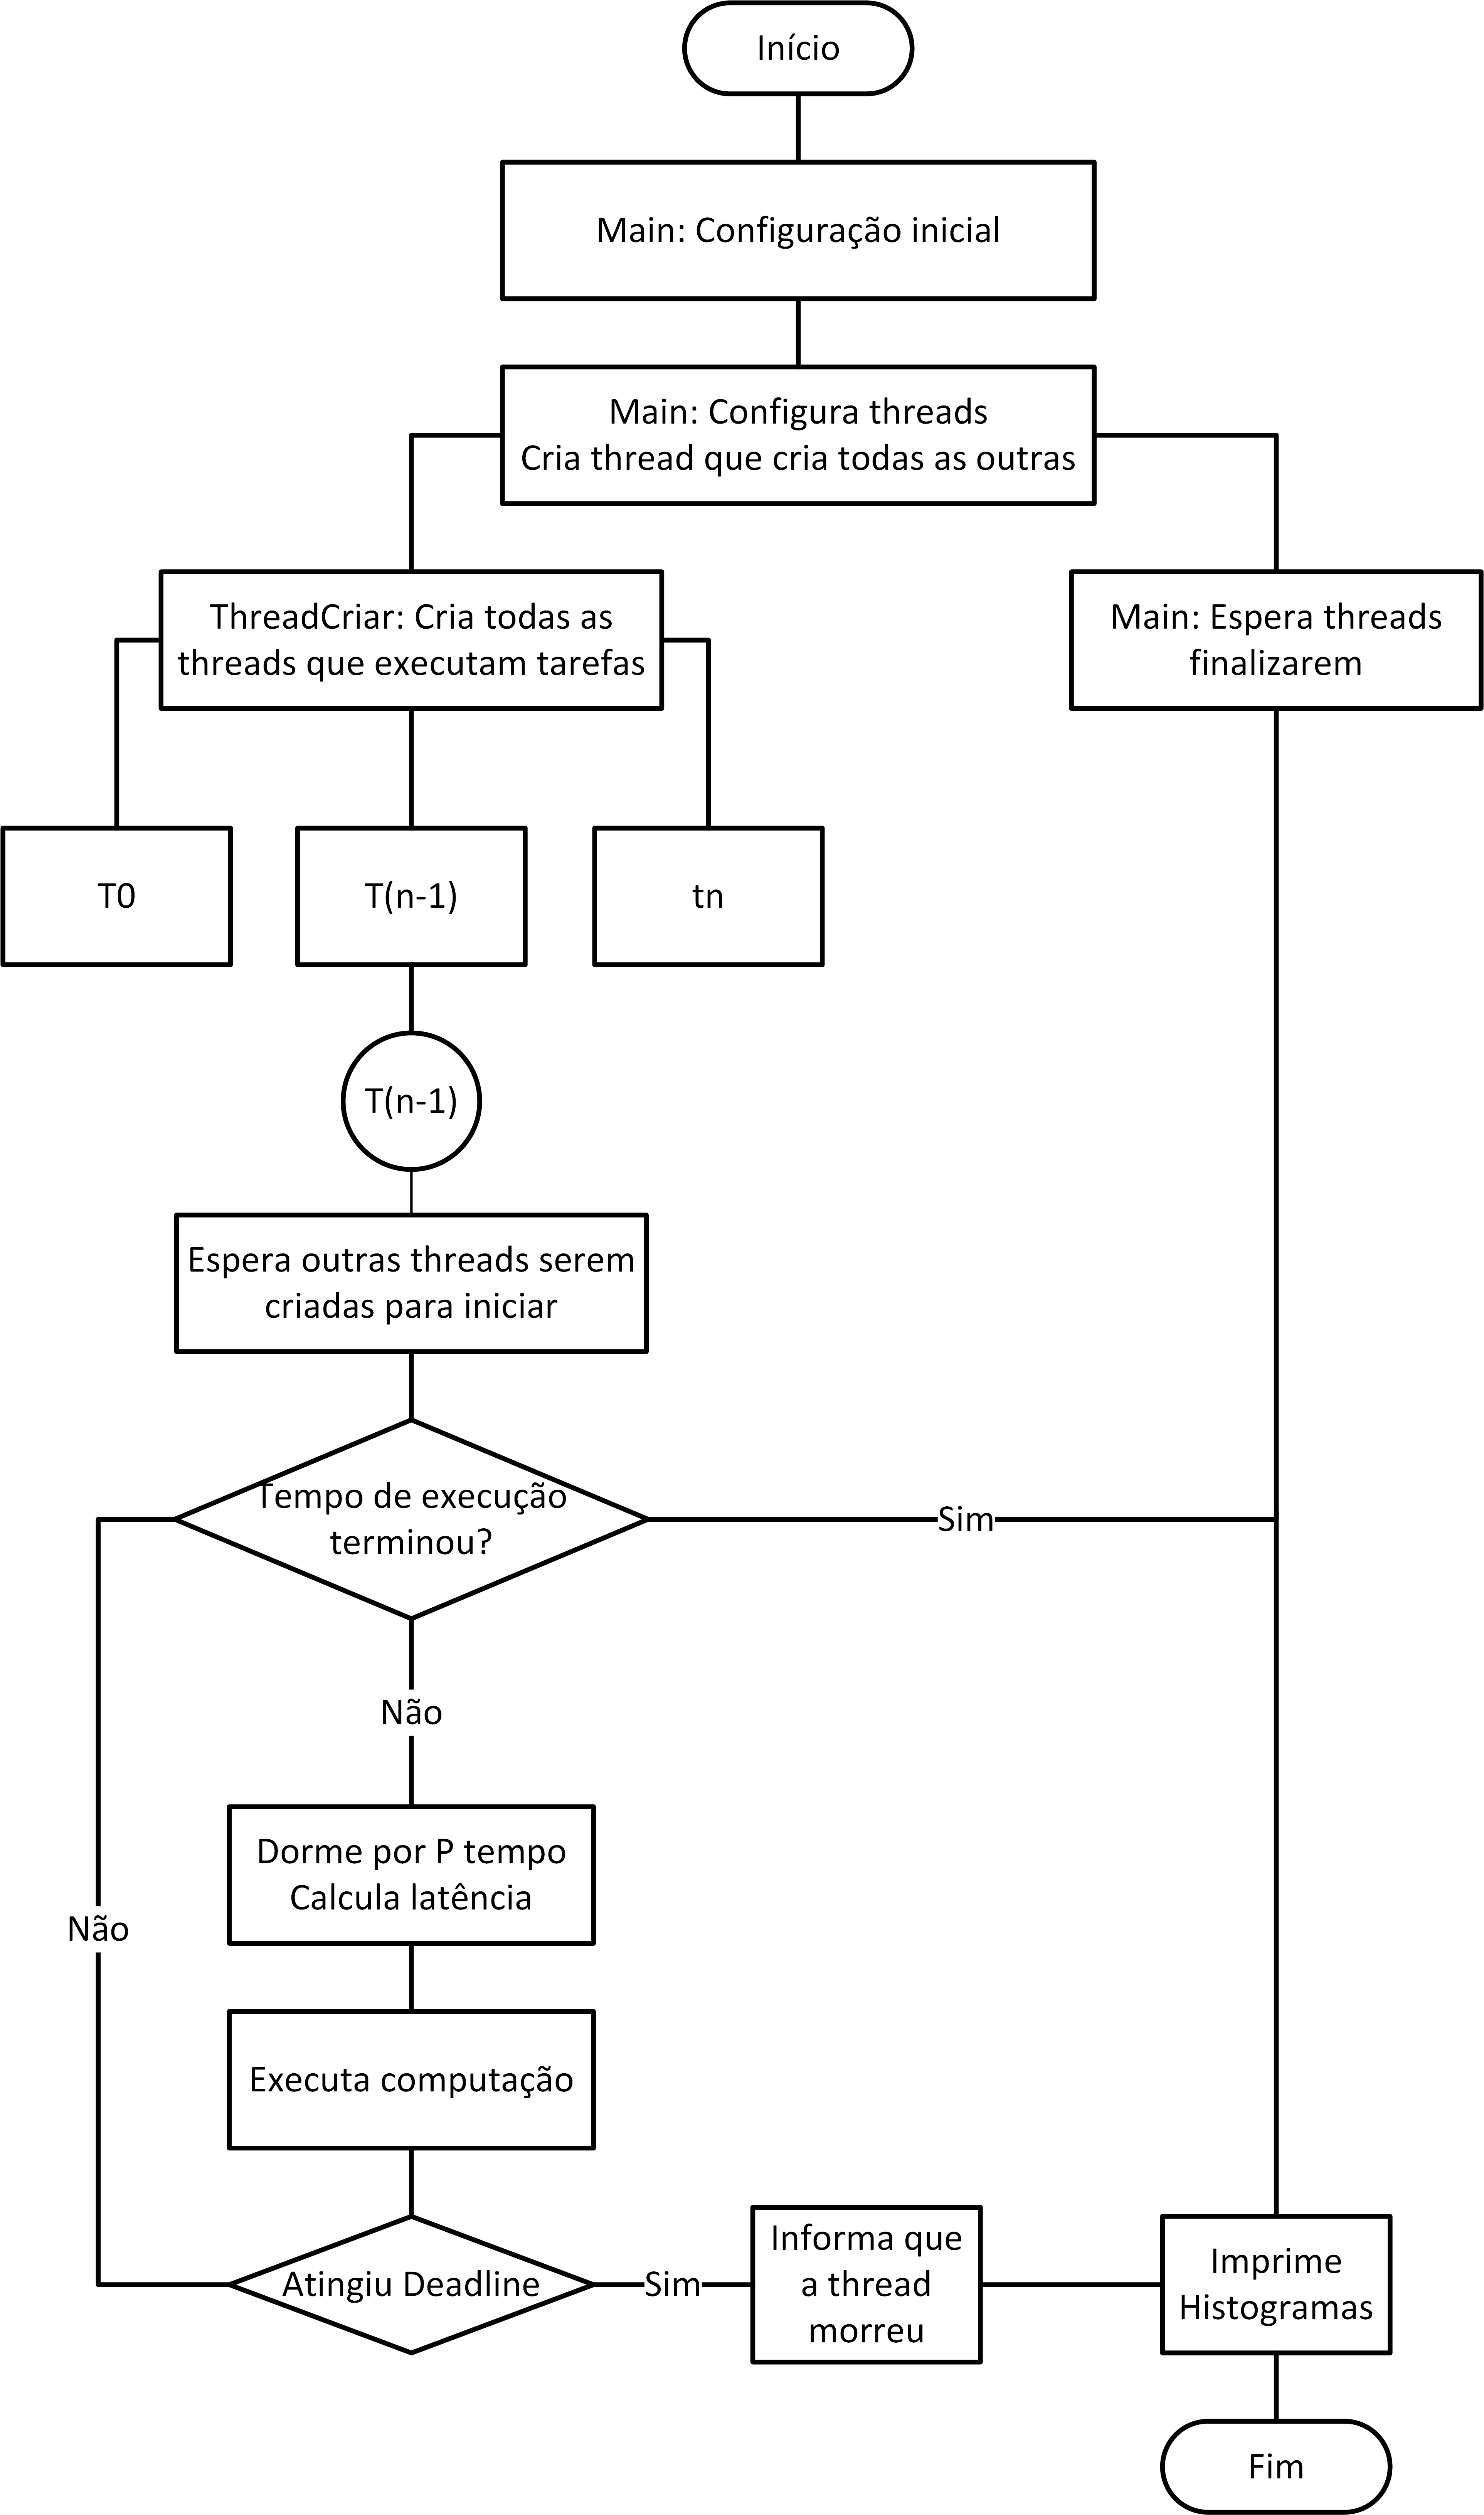
\includegraphics[scale=0.80]{FluxoProgramaDeTestes}
    \label{fluxograma}
\end{figure}

\chapter{\textit{Script} para inicialização do RTAI (rtai-init.bash)}
\label{cap:script}
\lstset{literate=
  {á}{{\'a}}1 {é}{{\'e}}1 {í}{{\'i}}1 {ó}{{\'o}}1 {ú}{{\'u}}1
  {Á}{{\'A}}1 {É}{{\'E}}1 {Í}{{\'I}}1 {Ó}{{\'O}}1 {Ú}{{\'U}}1
  {â}{{\^a}}1 {ê}{{\^e}}1 {î}{{\^i}}1 {ô}{{\^o}}1 {û}{{\^u}}1
  {Â}{{\^A}}1 {Ê}{{\^E}}1 {Î}{{\^I}}1 {Ô}{{\^O}}1 {Û}{{\^U}}1
  {ű}{{\H{u}}}1 {ő}{{\H{o}}}1 {ã}{{\H{a}}}1
  {ç}{{\c c}}1 {Ç}{{\c C}}1 {«}{{\guillemotleft}}1 {»}{{\guillemotright}}1
}
\lstset{language=bash}
\begin{lstlisting}[frame=single]
#!/bin/bash

# Carregando os módulos do RTAI
sudo insmod /usr/realtime/modules/rtai_hal.ko
sudo insmod /usr/realtime/modules/rtai_sched.ko
sudo insmod /usr/realtime/modules/rtai_fifos.ko
sudo insmod /usr/realtime/modules/rtai_sem.ko
sudo insmod /usr/realtime/modules/rtai_mbx.ko
sudo insmod /usr/realtime/modules/rtai_msg.ko
sudo insmod /usr/realtime/modules/rtai_shm.ko
sudo insmod /usr/realtime/modules/rtai_smi.ko
sudo insmod /usr/realtime/modules/latency_rt.ko

# Criando as variáveis para compilação
export CFLAGS=$(/usr/realtime/bin/./rtai-config --lxrt-cflags)
export LDFLAGS=$(/usr/realtime/bin/./rtai-config --lxrt-ldflags)
\end{lstlisting}

Para que as variáveis criadas pelo \textit{script} possam ser utilizadas por todos os usuários é preciso utilizar a notação ponto seguido por espaço:

\begin{lstlisting}[frame=single]
$ . rtai-init
\end{lstlisting}					

% !!! Fim do documento
\end{document}

